\documentclass[12pt]{article}
\usepackage{amsmath,latexsym,amsfonts,amssymb,graphicx,amsthm,epsfig,enumerate}
\usepackage{tikz,verbatim,tabularx} % adds charting fuctions
\newcolumntype{C}{>{\centering\arraybackslash}X}
\linespread{1.2}

%\pagestyle{empty}

\begin{document}
	\title{6 Man's Morris: 2AA4/2ME3 Assignment 1} %add title here
	\author{
		Gregory Smilski, 1404091\\
		Abigail Gaulin, 1327924\\
		Karl Knopf 1437217} 
	% add other necessary information here
	
	\maketitle
	\thispagestyle{empty}
	\newpage
	
	\section{Introduction}
	This document describes the java project 6 Men's Morris. 
	\subsection{Architecture}
	\begin{figure}[!h]
		\centering
		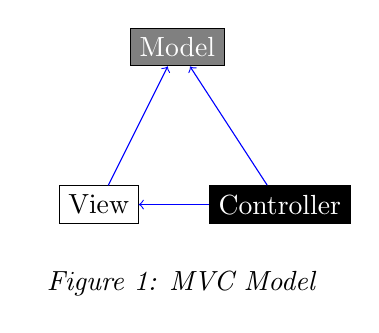
\begin{tikzpicture}
		% MVC Architecture
		\node[draw] (View) at (0,0) {View};
		\node[draw,fill=black,text=white] (Controller) at (2.3,0) {Controller};
		\node[draw,fill=gray,text=white] (Model) at (1,2) {Model};
		
		\draw[->,draw=blue] (View) to (Model);
		\draw[->,draw=blue] (Controller) to (View);
		\draw[->,draw=blue] (Controller) to (Model);
		\node at (1.0, -1.0) {\textit{ Figure 1: MVC Model}};
		
		\end{tikzpicture}
	\end{figure}
	This software uses MVC architecture in its design. MVC stands for Model, View, Controller, and is a design tool used in software development. The View contains all information the user sees, and interacts with the user. The Model contains all the data, and the Controller contains commands which modify the view and model. This architectural style is useful as it allows for modulation, and parts of the program can be modified without affecting any others.
	\subsection{Technologies}
	\begin{itemize}
		\item Java:  An object oriented programming language 
		\item Eclipse: It is an IDE used for the development and testing of software typically in Java
		\item Java Swing: A java toolkit designed to aid programmers in the creation of gui applications. This widget toolkit allows the programmer quick access to various predefined graphical objects, allowing the easy creation of a graphical interface.
		
	\end{itemize}
	\section{Modular Decomposition}
	% 4.1Description of the classes and modules and why they were used
		\begin{figure}[!h]
			\centering
			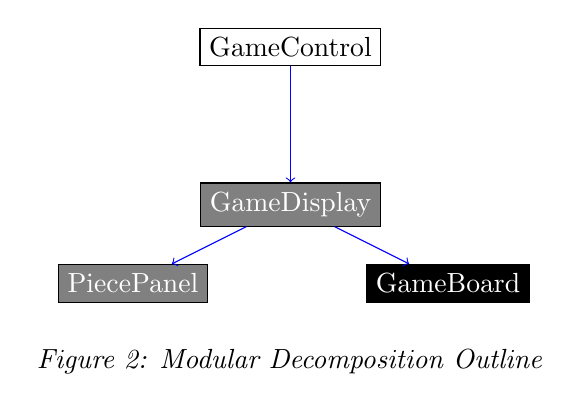
\begin{tikzpicture}
			% MVC Architecture
			\node[draw] (GameControl) at (1,3) {GameControl};
			\node[draw,fill=black,text=white] (GameBoard) at (3,0) {GameBoard};
			\node[draw,fill=gray,text=white] (GameDisplay) at (1,1) {GameDisplay};
			\node[draw,fill=gray,text=white] (PiecePanel) at (-1,0) {PiecePanel};
			
			\draw[->,draw=blue] (GameControl) to (GameDisplay);
			\draw[->,draw=blue] (GameDisplay) to (PiecePanel);
			\draw[->,draw=blue] (GameDisplay) to (GameBoard);
			\node at (1.0, -1.0) {\textit{Figure 2: Modular Decomposition Outline}};
			
			\end{tikzpicture}
		\end{figure}
	The modules chosen (as detailed in the Module Guide), were done so in order to make it straightforward for the 3 members involved in the project to code individually, and also to enforce modularity in the program. The GameDisplay, GameBoard and PiecePanel make up the View. The PiecePanel creates the tokens to take the user input, GameDisplay creates buttons to check or restart the game, and GameBoard displays the game data to the user. By dividing the View up in this way, if any of these functionalities need to be modified that can be done without affecting the other parts. The GameControl makes up the Controller. This controls the game logic, and is called by the View to make modifications to the game data based on user input. It makes sense for the Controller to be separate from the other modules, as any changes that are made to the game logic can be implemented without there being any change to what the user sees/interacts with, and likewise any changes to the user interface will not interfere with the game logic/data.
	\newpage
	\section{Module Guide}
	%4.2 For each module, a description of the interface and behaviors of each method
	\begin{itemize}
		   \item GameControl: Controls the game logic.
		   \begin{itemize}
		   	\item startboard: Initializes an instance of the board class. Initializes the arrays used to hold how many pieces in each position, and which players those pieces belong to. Additionally returns boolean value determining which player has the first turn.
		   	\item newpiece: Add a piece to the "current" and "teams" arrays in the given location.
		   	\item checkboard: Determines whether or not current board set-up is legal. Checks for stack errors (more than one peice on each ), or if a player has too many pieces on the board.
		   	\item visibleteam: Returns an int[][] of the top pieces of each position of the current board set-up.
		   	\item main: Runs program.
		   \end{itemize}
		   \item Error: A class to hold the variables of the checkerror output.
		   \begin{itemize}
		   	\item seterrortype: Sets the errortype variable to indicate the type of error present.
		   	\item seterrorarray: Sets the errorarray variable to indicate which positions a stack error is occuring at.
		   	\item setteamerror: Sets the teamerror variable to indicate which player has too many pieces on the board.
		   \end{itemize}
		   
		\item GameBoard : a class to hold the command that display the gameboard to the application window. 
			\begin{itemize}
			\item public int[][] visibleTeams: storage for the state of each game piece
			\item public boolean redTake: represents if red is the active player
			\item public boolean blueTake: represents if blue is the active player
			\item public int[][] sizingArray: represents the sizes of each level of game (inner or outer), used for scaling
			\item public double height: predetermined height of window
			\item public double width: predeteremined width of window
			\item public double size: predetermined size of window
			\item public GameBoard: default constructor for the gameboard.
			\end{itemize}
	\item PiecePanel(): It creates two interactive coloured circles where each player can draw their team's pieces from. When interacted with, it runs through a series of gates that which allow only certain players to add a piece.
	\item Piece() The constructor for piece object. Pieces should be added to the board during set up.
				\item GameDisplay(): The default constructor for the class GameDisplay, creates the panel and puts it into its place in the JFrame.
				\item GameDisplay(String): Creates a panel with two buttons that when pressed will either, depending on the button press, check if the positioning of pieces is legal or start a new game
				\begin{itemize}
					\item isButtonTake: A boolean to see if a button is selected
					\item isButtonRecieve: A boolean to see if a button is recieved
					
				\end{itemize}
	\end{itemize}
	\section{Traceability}
	% 4.5 A Description of each class
	% Tablular Expressions
	\begin{tabularx}{\linewidth}{|C|C|C|}
		Requirement & Module & Result \\
		\hline \\
		Random Player selected to go First & GameControl & random boolean generated to represent either player 1 or player 2 \\
		Setting up Board Array & GameControl & int[][] generated to hold values at each position on array. Initially, the array is empty, representing no disks on board. \\
		Checking if Board is Legal & GameControl & If there is more than one piece in a position, or too many pieces for a player on the board, an Error type is returned which holds value representing legality/error types present on board. \\
		Displaying an array as a Six Men's Morris Board &
		GameBoard & Game is Displayed as a panel on a jFrame, allows for user interaction \\ 
		Allowing the user to place a piece & GameBoard &
		User is able to select a location and place a piece \\
		The pieces used in the game are red and blue & GameBoard & The gameboard draws the pieces and restricts their colors to red and blue \\
		Starting with an empty board displayed & GameBoard & All of the spaces are initial empty (black) on the gameboard. \\
	\end{tabularx}
		\begin{tabularx}{\linewidth}{|C|C|C|}
			Requirement & Module & Result \\
			\hline \\
			
			New Game Button & GameDisplay & Allows user to select option to restart the board, will call GameControl. \\
			Check Button & GameDisplay  & Allows user to check if current board is legal, will call GameControl. \\
			User-Game Interaction & GameDisplay &Allows user to interact with game peices, make modifications to current board, will call GameControl. \\
	\end{tabularx}
	
	\section{Uses Relation}
	% A diagram and brief description describing why how the stuff interacts
			\begin{figure}[!h]
				\centering
				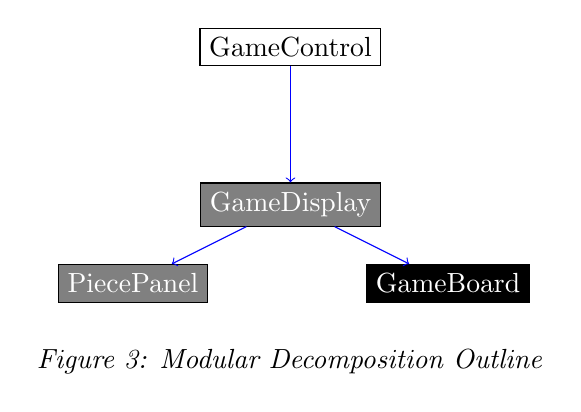
\begin{tikzpicture}
				% MVC Architecture
				\node[draw] (GameControl) at (1,3) {GameControl};
				\node[draw,fill=black,text=white] (GameBoard) at (3,0) {GameBoard};
				\node[draw,fill=gray,text=white] (GameDisplay) at (1,1) {GameDisplay};
				\node[draw,fill=gray,text=white] (PiecePanel) at (-1,0) {PiecePanel};
				
				\draw[->,draw=blue] (GameControl) to (GameDisplay);
				\draw[->,draw=blue] (GameDisplay) to (PiecePanel);
				\draw[->,draw=blue] (GameDisplay) to (GameBoard);
				\node at (1.0, -1.0) {\textit{Figure 3: Modular Decomposition Outline}};
				
				\end{tikzpicture}
			\end{figure}
	The View calls the Controller, which in turn modifies the Model. In the future, the View will initially take input from the user. Then, depending on which component was clicked, will call a corresponding method in the controller. Clicking either the red or blue piece will call the newpiece method in GameControl. Clicking the check button will call checkboard(), and clicking the start button will call startboard(). These methods will then modify the model through the manipulation of arrays. \\
	\newpage	
	\section{Testing}
	% A section on the testing of the software
	%Behavoir Table
	
	\begin{tabularx}{\linewidth}{|C|C|C|}
		What was Tested & What it did & Comments \\
		\hline \\
		GameControl: startboard & Printed out "current" and "teams" arrays & startboard is correctly setting up the "current" and "teams" arrays \\
		\hline \\
		GameControl: startboard & Printed out "first" boolean & "first" is correctly assigned random boolean values (on 3 separate tests was assigned true, false, and false) \\
		\hline \\
		GameControl: newpiece & Entered various input values (ie: 1,1,true) & Values were correctly entered into "current" and "teams" (ie: value of current[1][1] had 1 added to it, teams[1][1] had "a" added to it) \\
		\hline \\
		GameControl: checkboard & Ran function while no errors in array & Correctly returned no errors \\
		\hline \\
		GameControl: checkboard & Ran function while errors present & Correctly identified when too many pieces in a stack, and when a player has too many pieces on board \\
		\hline \\
		GameControl: visibleteam & Ran function with several different varieties of "teams" array (ie: when teams[0][1] = "abba") & Returned array was correct (ie: visibleteams[0][1] = "a" which is correct) \\
		\hline \\
	\end{tabularx}
	
	\begin{tabularx}{\linewidth}{|C|C|C|}
		What was Tested & What it did & Comments \\
		\hline \\
		GameBoard: GameBoard() & Display the board, allow for color change of disks & Constructor Method for the gameboard panel. Displays the board as a set of pieces. r \\
		GameBoard: GameBoard() Change Piece Color& Pieces Change color & The display was successfully able to read in the current color array. \\
	\end{tabularx}
	\begin{tabularx}{\linewidth}{|C|C|C|}
		What was Tested & What it did & Comments \\
		\hline 
		
		GameDisplay: GameDisplay() & Displayed panel in correct position in frame with buttons in correct positions in panel & GameDisplay is correctly setting up the panel \\
		GameDisplay: GameDisplay()& Clicked on "New Game?" Button,  printed "New Game!" in command line & GameDisplay is correctly running through correct output for the given input \\
		GameDisplay: GameDisplay() & Clicked on "Check!" Button, printed "Is is correct?" in command line & GameDisplay is correctly running through corect output for the given input \\
		PiecePanel: PiecePanel() & Displayed panel in correct position in frame with circle tokens in correct position in panel & PiecePanel is correctly setting up the panel \\
		PiecePanel: PiecePanel() & Clicked on Red Circle, Displayed "add red?" & PiecePanel is giving the crect output for the given input and is ready to add a red piece to the board \\
	\end{tabularx}
	\begin{tabularx}{\linewidth}{|C|C|C|}
		What was Tested & What it did & Comments \\
		\hline 
		PiecePanel: PiecePanel() &  Clicked on Blue Circle, Displayed "add blue?" & PiecePanel is giving the corect output for the given input and is ready to add a blue piece to the board \\
		PiecePanel: PiecePanel()  , Clicked on Red Circle, then white circle & White Cirtcle turned red & PiecePanel is giving the corect output for the given input and should add a red piece to the board \\
		PiecePanel: PiecePanel()  , Clicked on Red Circle, then white circle that has been coloured red & No output occurred & PiecePanel is giving the corect output for the given input and any additional red peices were not added not on their turn \\
		PiecePanel: PiecePanel()  , Clicked on Blue Circle, then white circle that has been coloured red & The red coloured white circle turned blue & PiecePanel is giving the corect output for the given input and a blue peice shoule be added \\
		PiecePanel: PiecePanel()  , Clicked on Blue Circle, then white circle & White Circle turned Blue & PiecePanel is giving the corect output for the given input and should add a blue piece to the board \\
		PiecePanel: PiecePanel()  , Clicked on Blue Circle, then white circle that has been coloured blue & No output occurred & PiecePanel is giving the corect output for the given input and any additional red peices were not added not on their turn \\
		PiecePanel: PiecePanel()  , Clicked on Red Circle, then white circle that has been coloured blue & The blue coloured white circle turned red & PiecePanel is giving the corect output for the given input and a red piece should be added \\
	\end{tabularx}
	\section{Discussion}
	%4.6 Internal review/ evaluation of design
	The design roughly follows the MVC format. The View is implented in GameDisplay, GameBoard and PiecePanel. The Controller is implemented in GameControl, which also modifies the Model. All of these parts should meet their individual requirements as shown in the Testing section.
	At present, these parts do not function together, and the connectivity of these parts will be implemented later on.
	\subsection{Anticipated Changes}
	% what was designed in anticipation of changes
	\begin{itemize}
	\item    GameControl: Will be able to track movement of pieces in the "current" and "teams" arrays (at present, can only add new pieces in). Arrays were designed to contain variables that could be modified in the future to reflect these changes.
	    In the future, the GameControl could be easily used with different dimensions (ie 8 Men's Morris).  
	\item    Error: Class designed to hold variables needed to explain what type of error is present to user of program. Returns a integer indicating the type of error, and a int[][], indicating the locations of any stack errors. Due to the design of a separate error case, if any other error types are required in the future, it will be simple to add them in.
	\item	As it currently stands, the class PiecePanel runs part of what should be in GameControl when it checks which team should be allowed to play a piece. In later versions, PiecePanel will communicate with GameControl in order to implement proper MVC design. Additionally, PiecePanel does not add actual piece objects to the board. Instead, it simply changes the colour of a test board location located between the two coloured circles. Proper adding of pieces to the board will be implemented in later versions. Also, pieces are not currently created as actual objects that can be added to the board as intended with the Piece class, so this will be changed. Finally, GameBoard does not communicate with GameControl to check if pieces are in legal locations or to start a new game. This will be implemented in later versions.
	\item Gameboard: In the near future, Gameboard() will be able to interact with the other module, using the information stored in GameControl and GameDisplay. Gameboard will also be able to succesfully check if a move is legal and be able to reset the board based on exteral commands. Some sections will be removed once they are redundant.
	\end{itemize}
	
\end{document}